\section{PHD Filter}

\subsection*{PHD Filter}\begin{frame}[t]\frametitle{PHD Filter}
    \begin{itemize}
        \item Assume that the expected number of objects in the area $S$ is:
            \begin{equation*}
                E[| \Xi \cap S |] = \int_S \nu_\Xi(\mathbf{x}) \mathrm{d} \mathbf{x}.
            \end{equation*}
            \begin{itemize}
                \item $\nu_\Xi(\mathbf{x})$ is called the intensity (PHD) function.
                \item It is a distribution but non-normalized.
            \end{itemize}
        \begin{center}
            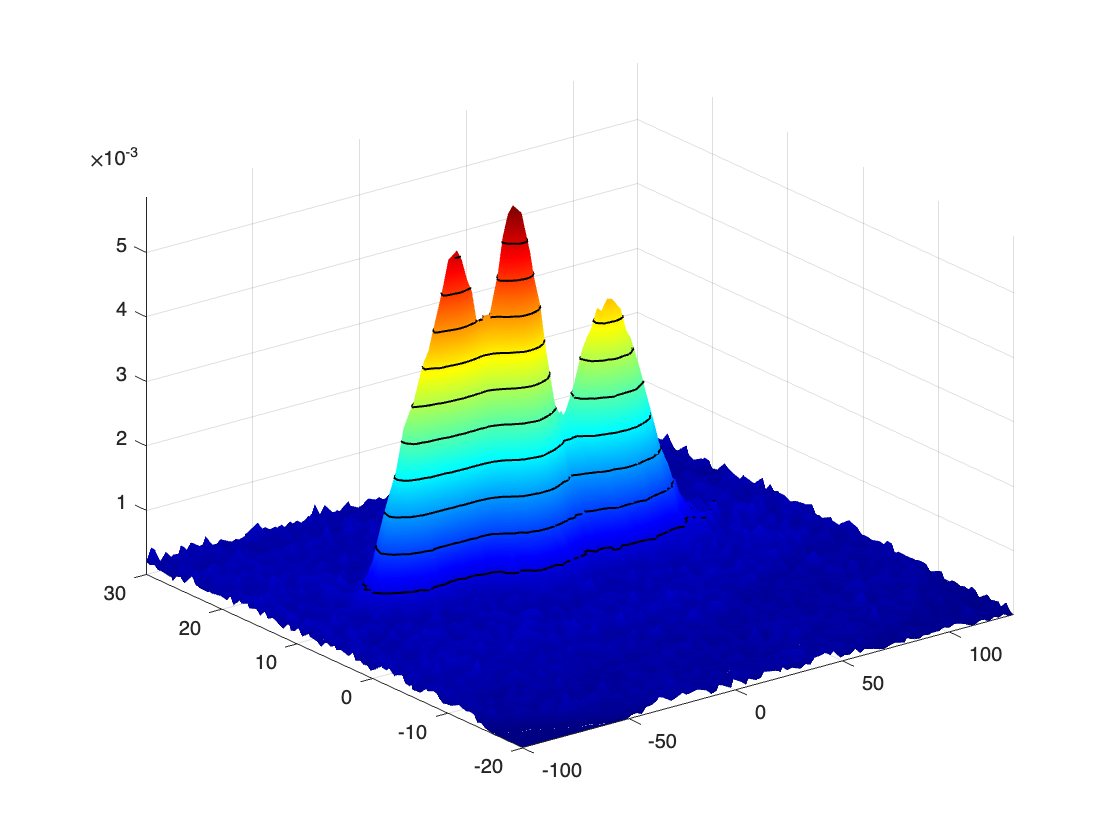
\includegraphics[width=0.5\linewidth]{pic/phd-fun.png}
        \end{center}
        \pause
        \item The PHD filter computes only the first-order moment, not the full posterior.
    \end{itemize}
\end{frame}

\begin{frame}{GM-PHD Filter}
    \begin{itemize}
        \item For Gaussian-linear cases, the GM-PHD filter is used.
        \pause
        \item The dynamics of a single object is modeled using the linear Kalman filter.
        \pause
        \item The noise is modeled as a Poisson Point Process.
        \pause
        \item At a single time step, the complexity is only $\mathcal O(mn)$, where
            \begin{itemize}
                \item $n$ is the number of targets at time step $k$,
                \item $m$ is the number of measurements at time step $k$.
            \end{itemize}
        \pause
        \item Target estimates are the mean vectors of the highest peaks.
        \pause
        \item The intensity is represented using a Gaussian mixture.
        \pause
        \item \alert{Consider this: What if we could directly modify the intensity to incorporate information from other sensors?}
    \end{itemize}
\end{frame}
